\subsection{W\"urstchen}
In Section~\ref{heading:subsection:stable_diffusion} we describe the approach
of a \emph{Latent Diffusion Model} (LDM) which was introduced,
by Rombach et al.~\cite{rombach2022stablediffusion} in 2022. The LDM methods
generates images by first encoding the semantics of a prompt into a token and
introduces this information into a noisy latent image by denoising
it based on the token. Lastly the latent representation is decoded into the
pixel space. By mostly navigating in low dimensional latent spaces and
utilizing the U-Net to slowly induce semantics into the representation, this
approach is able to yield high resolution images~\cite{rombach2022stablediffusion}.
This improvement in image quality has a disadvantage: the time the models take
to train. For example an important model is Stable Diffusion (SD), the version
1.4 takes 150,000 GPU hours~\cite{rombach2022sd_1_4} while version 2.1 which
grants an upgrade in image quality has a further increased training time of
200,000 GPU hours~\cite{rombach2023sd_2_1}. A high image resolution comes with
an increased image complexity leading to a higher data-intensive training and
high computational costs. Thus, Pernias et al.~\cite{pernias2024wrstchen}
introduce \emph{W\"urstchen}. An approach that tries to lower the training time
and computational cost, by splitting the training process into three parts and
mostly computing in small latent spaces.\\

This section aims to describe the methods used by W\"urstchen based on the work
of Pernias et al.~\cite{pernias2024wrstchen}. First we describe the VQGAN by
Esser et al.~\cite{esser2021tamingtransformershighresolutionimage} as this is
the foundation of W\"urstchen. Then, we continue to describe the general
architecture and the detailed training process of the model. Finally, we shed
light onto the image generation process of W\"urstchen.

\subsubsection{VQGAN}
The \emph{Vector Quantized Generative Adversarial Network} (VQGAN) was introduced by
Esser et al~\cite{esser2021tamingtransformershighresolutionimage} in 2021 and
builds on the \emph{Vector Quantized Variational Autoencoder}
model~\cite{vdOord2017NeuralDiscreteRepresentationLearning}. The VQGAN combines
the strength of \emph{Convolutional Neural Networks} (CNN) to exploit knowledge
of local features and the strength of autoregressive transformer architectures
to model long-range relations. As Esser et al. introduce the VQGAN uses several
CNNs during training. The first CNN is called the Encoder which is able to
compress a picture $x$ into the compressed version $\hat{z}$. Afterward,
the VQGAN utilizes the quantization $\boldsymbol{q}[\cdot]$ using a
perceptually rich and discrete codebook $\mathcal{Z}$ to create the quantized
latent representation,
\begin{equation}
    z_{\boldsymbol{q}} = \boldsymbol{q}(\hat{z}) :=\underset{z_{\boldsymbol{k}}\in\mathcal{Z}}{\arg\min}||\hat{z}_{ij} - z_{\boldsymbol{k}}||,
\end{equation}
by replacing the spatial representation $\hat{z}_{ij}$ with the closest
codebook entry $z_{\boldsymbol{k}}$. The latent representation
$z_{\boldsymbol{q}}$ is a sequence of the entries of the codebook $\mathcal{Z}$.
Finally, the Decoder CNN reconstructs the image $x$ using the quantized latent
representation $z_{\boldsymbol{q}}$. To create a rich codebook a patch-based
discriminator CNN is introduced to find the differences between the real and
reconstructed images. An autoregressive transformer model then makes use of the
codebook to generate high-resolution synthetic images.

\subsubsection{Architecture and Structure}
\begin{figure}[t]
    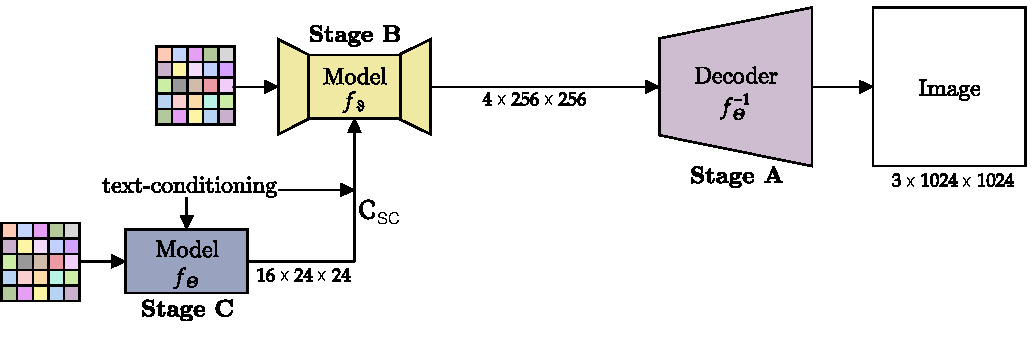
\includegraphics[width=\textwidth]{assets/wuerstchen_arch.pdf}
    \caption{Visualization of the W\"urstchen architecture, introduced by
        Pernias et al.~\cite{pernias2024wrstchen}. It shows that the first stage C
        creates a highly compressed representation from noise and text-conditioning.
        Both this representation and the text-prompt are then utilized as conditioning by stage B
        to create a higher dimensional latent representation. Lastly, the decoder
        in stage A generates an image from this latent representation.}
    \label{fig:wuerstchen:arch}
\end{figure}
In 2024 Pernias et al.~\cite{pernias2024wrstchen} introduce \emph{W\"urstchen}.
With this method they set out to decrease the computation cost and training
time of image generation models which are based on latent diffusion~\cite{rombach2022stablediffusion}.
W\"urstchen is build up from three stages. The first stage, Stage C, comprises
a text-conditional diffusion model $f_\Theta$ that operates on a
low-dimensional latent space with a compression ratio of 42:1. Due to this,
$f_\Theta$ does not perform any downsampling as the authors decided that the
typical U-Net structure would do harm to the image quality. The next stage,
Stage B, a diffusion model $f_\vartheta$, utilizing the U-Net architecture and
conditioned on both the text-prompt and the embeddings $\mathcal{C}_{\text{SC}}$
of the low-dimensional latent representation generates a higher dimensional
latent representation with a compression ratio of 4:1. This latent space is
generated by a VQGAN during training. Stage A of W\"urstchen consists of the decoder $f_\theta^{-1}$
of this VQGAN which reconstructs the image from the latent representation
generated in Stage B.
% introduce training time and cost reduction through calculation in lower dimensions and split in architecture
% first model encodes prompt into a latent representation of a very low compression 42:1
% second model uses this latent representation to navigate in a less compressed latent space with compression ratio of 4:1
% last model is the decoder branch of an VQGAN that translates the latent representation into the pixel space

\subsubsection{Training}

\paragraph*{Stage A}

\paragraph*{Stage B}

\paragraph*{Stage C}

\subsubsection{Image Generation}